\documentclass{standalone}
\usepackage[utf8]{inputenc}
\usepackage{pgfplots}
\DeclareUnicodeCharacter{2212}{−}
\usepgfplotslibrary{groupplots,dateplot}
\usetikzlibrary{patterns,shapes.arrows}
\pgfplotsset{compat=newest}
\begin{document}
% This file was created with tikzplotlib v0.10.1.post13.
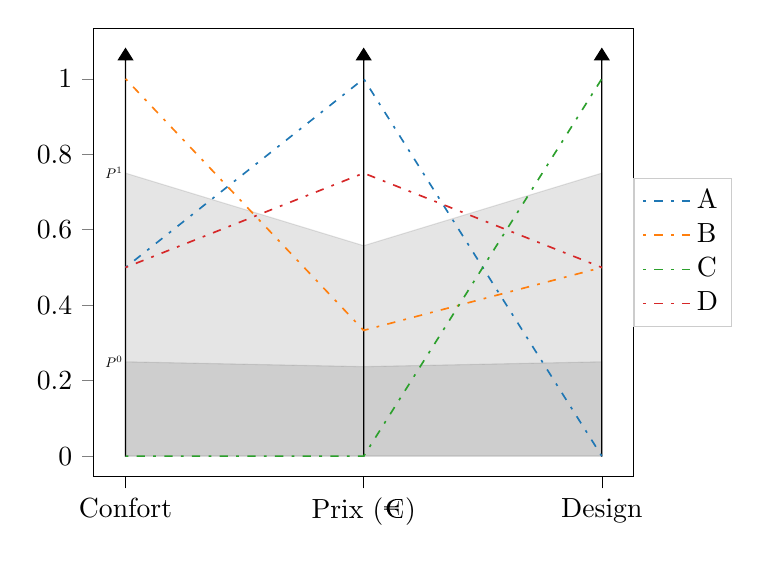
\begin{tikzpicture}

\definecolor{crimson2143940}{RGB}{214,39,40}
\definecolor{darkgrey176}{RGB}{176,176,176}
\definecolor{darkorange25512714}{RGB}{255,127,14}
\definecolor{forestgreen4416044}{RGB}{44,160,44}
\definecolor{lightgrey204}{RGB}{204,204,204}
\definecolor{steelblue31119180}{RGB}{31,119,180}

\begin{axis}[
legend cell align={left},
legend style={
  fill opacity=0.8,
  draw opacity=1,
  text opacity=1,
  at={(1,0.5)},
  anchor=west,
  draw=lightgrey204
},
tick align=outside,
tick pos=left,
x grid style={darkgrey176},
xmin=-0.133, xmax=2.133,
xtick style={color=black},
xtick={0,1,2},
xticklabels={Confort,Prix (€),Design},
ymin=-0.054, ymax=1.134
]
\path [draw=black, fill=black, opacity=0.1]
(axis cs:0,0)
--(axis cs:0,0.25)
--(axis cs:1,0.237179487179487)
--(axis cs:2,0.25)
--(axis cs:2,0)
--(axis cs:2,0)
--(axis cs:1,0)
--(axis cs:0,0)
--cycle;

\path [draw=black, fill=black, opacity=0.1]
(axis cs:0,0)
--(axis cs:0,0.75)
--(axis cs:1,0.557692307692308)
--(axis cs:2,0.75)
--(axis cs:2,0)
--(axis cs:2,0)
--(axis cs:1,0)
--(axis cs:0,0)
--cycle;

\path [draw=black, fill=black]
(axis cs:0,1.08)
--(axis cs:0.03,1.05)
--(axis cs:0.0005,1.05)
--(axis cs:0.0005,0)
--(axis cs:-0.0005,0)
--(axis cs:-0.0005,1.05)
--(axis cs:-0.03,1.05)
--cycle;
\path [draw=black, fill=black]
(axis cs:1,1.08)
--(axis cs:1.03,1.05)
--(axis cs:1.0005,1.05)
--(axis cs:1.0005,0)
--(axis cs:0.9995,0)
--(axis cs:0.9995,1.05)
--(axis cs:0.97,1.05)
--cycle;
\path [draw=black, fill=black]
(axis cs:2,1.08)
--(axis cs:2.03,1.05)
--(axis cs:2.0005,1.05)
--(axis cs:2.0005,0)
--(axis cs:1.9995,0)
--(axis cs:1.9995,1.05)
--(axis cs:1.97,1.05)
--cycle;
\addplot [semithick, steelblue31119180, dash pattern=on 1pt off 3pt on 3pt off 3pt]
table {%
0 0.5
1 1
2 0
};
\addlegendentry{A}
\addplot [semithick, darkorange25512714, dash pattern=on 1pt off 3pt on 3pt off 3pt]
table {%
0 1
1 0.333333333333333
2 0.5
};
\addlegendentry{B}
\addplot [semithick, forestgreen4416044, dash pattern=on 1pt off 3pt on 3pt off 3pt]
table {%
0 0
1 0
2 1
};
\addlegendentry{C}
\addplot [semithick, crimson2143940, dash pattern=on 1pt off 3pt on 3pt off 3pt]
table {%
0 0.5
1 0.75
2 0.5
};
\addlegendentry{D}
\draw (axis cs:0,0.25) ++(-1pt,0pt) node[
  scale=0.5,
  fill=none,
  draw=none,
  line width=0.4pt,
  inner sep=0pt,
  rounded corners,
  anchor=east,
  text=black,
  rotate=0.0
]{$P^0$};
\draw (axis cs:0,0.75) ++(-1pt,0pt) node[
  scale=0.5,
  fill=none,
  draw=none,
  line width=0.4pt,
  inner sep=0pt,
  rounded corners,
  anchor=east,
  text=black,
  rotate=0.0
]{$P^1$};
\draw (axis cs:0,1.2) node[
  scale=0.5,
  fill=white,
  draw=lightgrey204,
  line width=0.4pt,
  inner sep=3pt,
  fill opacity=1,
  rounded corners,
  anchor=base west,
  text=black,
  rotate=0.0
]{Lexicographic order : $P^0 \rightarrow P^1$};
\end{axis}

\end{tikzpicture}

\end{document}